\documentclass[portrait,a0paper,fontscale=0.277]{baposter}

\usepackage{calc}
\usepackage{graphicx}
\usepackage{amsmath}
\usepackage{amssymb}
\usepackage{relsize}
\usepackage{multirow}
\usepackage{rotating}
\usepackage{bm}
\usepackage{url}

%\usepackage{graphicx}
\usepackage{multicol}

%\usepackage{times}
%\usepackage{helvet}
%\usepackage{bookman}
\usepackage{palatino}

\newcommand{\captionfont}{\footnotesize}

\graphicspath{{images/}{../images/}}
\usepackage{tikz}
\usetikzlibrary{arrows,shapes,calc}

\newcommand{\SET}[1]  {\ensuremath{\mathcal{#1}}}
\newcommand{\MAT}[1]  {\ensuremath{\boldsymbol{#1}}}
\newcommand{\VEC}[1]  {\ensuremath{\boldsymbol{#1}}}
\newcommand{\Video}{\SET{V}}
\newcommand{\video}{\VEC{f}}
\newcommand{\track}{x}
\newcommand{\Track}{\SET T}
\newcommand{\LMs}{\SET L}
\newcommand{\lm}{l}
\newcommand{\PosE}{\SET P}
\newcommand{\posE}{\VEC p}
\newcommand{\negE}{\VEC n}
\newcommand{\NegE}{\SET N}
\newcommand{\Occluded}{\SET O}
\newcommand{\occluded}{o}

%%%%%%%%%%%%%%%%%%%%%%%%%%%%%%%%%%%%%%%%%%%%%%%%%%%%%%%%%%%%%%%%%%%%%%%%%%%%%%%%
%%%% Some math symbols used in the text
%%%%%%%%%%%%%%%%%%%%%%%%%%%%%%%%%%%%%%%%%%%%%%%%%%%%%%%%%%%%%%%%%%%%%%%%%%%%%%%%

%%%%%%%%%%%%%%%%%%%%%%%%%%%%%%%%%%%%%%%%%%%%%%%%%%%%%%%%%%%%%%%%%%%%%%%%%%%%%%%%
% Multicol Settings
%%%%%%%%%%%%%%%%%%%%%%%%%%%%%%%%%%%%%%%%%%%%%%%%%%%%%%%%%%%%%%%%%%%%%%%%%%%%%%%%
\setlength{\columnsep}{1.5em}
\setlength{\columnseprule}{0mm}

%%%%%%%%%%%%%%%%%%%%%%%%%%%%%%%%%%%%%%%%%%%%%%%%%%%%%%%%%%%%%%%%%%%%%%%%%%%%%%%%
% Save space in lists. Use this after the opening of the list
%%%%%%%%%%%%%%%%%%%%%%%%%%%%%%%%%%%%%%%%%%%%%%%%%%%%%%%%%%%%%%%%%%%%%%%%%%%%%%%%
\newcommand{\compresslist}{%
\setlength{\itemsep}{1pt}%
\setlength{\parskip}{0pt}%
\setlength{\parsep}{0pt}%
}

%%%%%%%%%%%%%%%%%%%%%%%%%%%%%%%%%%%%%%%%%%%%%%%%%%%%%%%%%%%%%%%%%%%%%%%%%%%%%%
%%% Begin of Document
%%%%%%%%%%%%%%%%%%%%%%%%%%%%%%%%%%%%%%%%%%%%%%%%%%%%%%%%%%%%%%%%%%%%%%%%%%%%%%

\begin{document}
\typeout{Poster Starts}
\background{
\begin{tikzpicture}[remember picture,overlay]%
\draw (current page.north west)+(-2.62em,2.4em) node[anchor=north west] {
\includegraphics[height=1.\textheight]{PDFTemplate}};
\end{tikzpicture}%
}

%%%%%%%%%%%%%%%%%%%%%%%%%%%%%%%%%%%%%%%%%%%%%%%%%%%%%%%%%%%%%%%%%%%%%%%%%%%%%%
%%% Here starts the poster
%%%---------------------------------------------------------------------------
%%% Format it to your taste with the options
%%%%%%%%%%%%%%%%%%%%%%%%%%%%%%%%%%%%%%%%%%%%%%%%%%%%%%%%%%%%%%%%%%%%%%%%%%%%%%
% Define some colors

%\definecolor{lightblue}{cmyk}{0.83,0.24,0,0.12}
\definecolor{lightblue}{rgb}{0.2667,0.2706,0.4627}
\definecolor{darkblue}{rgb}{0.5490,0.2039,0.8353}
\definecolor{lightpurple}{rgb}{0.8,0.8,1}

\definecolor{silver}{cmyk}{0,0,0,0.3}
\definecolor{yellow}{cmyk}{0,0,0.9,0.0}
\definecolor{reddishyellow}{cmyk}{0,0.22,1.0,0.0}
\definecolor{black}{cmyk}{0,0,0.0,1.0}
\definecolor{darkYellow}{cmyk}{0,0,1.0,0.5}
\definecolor{darkSilver}{cmyk}{0,0,0,0.1}
\definecolor{lightyellow}{cmyk}{0,0,0.3,0.0}
\definecolor{lighteryellow}{cmyk}{0,0,0.1,0.0}
\definecolor{lightestyellow}{cmyk}{0,0,0.05,0.0}
\definecolor{thalesMarine}{cmyk}{0.95,0.90,0,0.3}
\definecolor{thalesTurquoise}{cmyk}{0.76,0,0.1,0}
%\definecolor{midnightblue}{cmyk}{1,1,0,0.5}
\definecolor{midnightblue}{cmyk}{0.78,0.78,0,0.56}
\definecolor{bloodred}{cmyk}{0,1,1,0.6}
\definecolor{lavender}{cmyk}{0.08,0.08,0,0.02}
\definecolor{pine}{cmyk}{0.18,0.0,0.77,0.69}
\definecolor{olive}{cmyk}{0.24,0.0,0.76,0.45}
\definecolor{pinegreen}{cmyk}{1.0,0.0,1.0,1.0}
\definecolor{clover}{cmyk}{0.61,0.0,0.47,0.37}
\definecolor{indianred}{cmyk}{0.0,0.58,0.58,0.0}
\definecolor{mistyrose}{cmyk}{0.0,0.31,0.32,0.6}
%\definecolor{mistyrose}{cmyk}{0.0,0.11,0.12,0.2}
\definecolor{deeppurple}{cmyk}{0.0,0.81,0.4,0.67}

 
% Draw a video
%% \newlength{\FSZ}
%% \newcommand{\drawvideo}[3]{% [0 0.25 0.5 0.75 1 1.25 1.5]
%%    \noindent\pgfmathsetlength{\FSZ}{\linewidth/#2}
%%    \begin{tikzpicture}[outer sep=0pt,inner sep=0pt,x=\FSZ,y=\FSZ]
%%    \draw[color=lightblue!50!black] (0,0) node[outer sep=0pt,inner sep=0pt,text width=\linewidth,minimum height=0] (video) {\noindent#3};
%%    \path [fill=lightblue!50!black,line width=0pt] 
%%      (video.north west) rectangle ([yshift=\FSZ] video.north east) 
%%     \foreach \x in {1,2,...,#2} {
%%       {[rounded corners=0.6] ($(video.north west)+(-0.7,0.8)+(\x,0)$) rectangle +(0.4,-0.6)}
%%     }
%% ;
%%    \path [fill=lightblue!50!black,line width=0pt] 
%%      ([yshift=-1\FSZ] video.south west) rectangle (video.south east) 
%%     \foreach \x in {1,2,...,#2} {
%%       {[rounded corners=0.6] ($(video.south west)+(-0.7,-0.2)+(\x,0)$) rectangle +(0.4,-0.6)}
%%     }
%% ;
%%    \foreach \x in {1,...,#1} {
%%      \draw[color=lightblue!50!black] ([xshift=\x\linewidth/#1] video.north west) -- ([xshift=\x\linewidth/#1] video.south west);
%%    }
%%    \foreach \x in {0,#1} {
%%      \draw[color=lightblue!50!black] ([xshift=\x\linewidth/#1,yshift=1\FSZ] video.north west) -- ([xshift=\x\linewidth/#1,yshift=-1\FSZ] video.south west);
%%    }
%%    \end{tikzpicture}
%% }

\hyphenation{resolution occlusions}
%%


% macros from ijcai2013 paper
\def\dae{{\em Divide-and-Evolve}}
\def\DAE{{\sc DaE}}
\def\DAEX{{\sc DaE$_{\text{X}}$}}
%\def\DAEYAHSP{{\sc DaE$_{\text{YAHSP}}$}}
\newcommand{\DAEYAHSP}{{\sc DaE$_{\text{YAHSP}}$}}
\def\PARADISEO{{\sc ParadisEO-MOEO}}
\def\YAHSP{{\sc YAHSP}}
\def\CPT{{\sc CPT}}
\def\modae{{\em Multiobjective Divide-and-Evolve}}
\def\MODAE{{\sc MO-DaE}}
\newcommand{\MODAEYAHSP}{{\sc MO-DaE$_{\text{YAHSP}}$}}
\newcommand{\MODAEX}{{\sc MO-DaE$_{\text{X}}$}}
\newcommand{\MOLPG}{{\sc MO-LPG}}
\def\ZENO{{\sc Zeno}}
\def\MULTIZENO{{\sc MultiZeno}}
\def\PARAMILS{{\sc ParamILS}}
\def\IBEAH{{\sc IBEA$_{\text{H}}$}}

\def\WMAKESPAN{{W-makespan}}
\def\WCOST{{W-cost}}

\newcommand{\ZENOTRAVEL}{{\sc ZenoTravel}}
\newcommand{\OPENSTACKS}{{\sc Openstacks}}
\newcommand{\ELEVATORS}{{\sc Elevators}}
\newcommand{\CREWPLANNING}{{\sc CrewPlanning}}
\newcommand{\FLOORTILE}{{\sc Floortile}}
\newcommand{\PARCPRINTER}{{\sc ParcPrinter}}

\newcommand{\mycomments}[1]{\textcolor{red}{#1}}
% \newcommand{\mycomments}[1]{~}

% bullets for itemize lists
\renewcommand{\labelitemi}{$\bullet$}
\renewcommand{\labelitemii}{$\cdot$}
\renewcommand{\labelitemiii}{$\diamond$}
\renewcommand{\labelitemiv}{$\ast$}


\begin{poster}%
  % Poster Options
  {
  % Show grid to help with alignment
  grid=false,
  % Column spacing
  colspacing=1em,
  % Color style
	%bgColorOne=lighteryellow,
  %bgColorTwo=lightestyellow,
bgColorOne=white,
  %bgColorTwo=white,
%bgColorTwo=lightpurple,
%bgColorTwo=darkSilver,
bgColorTwo=lavender,
%bgColorTwo=reddishyellow,
	%bgColorTwo=silver,
  borderColor=mistyrose,
  headerColorOne=pine,
  headerColorTwo=olive,
  headerFontColor=white,
  boxColorOne=white,
  boxColorTwo=lightblue,
  % Format of textbox
  textborder=roundedleft,
  % Format of text header
  eyecatcher=true,
	%eyecatcher=false,
  headerborder=closed,
  headerheight=0.1\textheight,
%  textfont=\sc, An example of changing the text font
  headershape=roundedright,
  headershade=shadelr,	
	%headerfont=\Large\bf\textsc, %Sans Serif
	headerfont=\Large\bf, %Sans Serif
%  textfont={\color{deeppurple}\setlength{\parindent}{0em}},
  textfont={\color{pinegreen}\setlength{\parindent}{0em}},
%  textfont={\setlength{\parindent}{1.5em}},
%headerFontColor=thalesMarine,
  %boxshade=plain,
	boxshade=none,
  %background=none,
  %background=shadetb,
  %background=plain,
	background=user,
  linewidth=2pt
  }
  % Eye Catcher
	{
	\makebox[10em]{ }
	}
	%{
\includegraphics[scale=0.3]{PDFTemplate}}
  %{\includegraphics[scale=0.3]{logo_gecco2013}}
  %{\includegraphics[height=5em]{logo_lri}}
  % Title
{\color{purple} Pareto-Based Multiobjective\\ AI Planning\vspace{0.3em}}
  % Authors
%{\color{bloodred} \large Mostepha-Redouane Khouadjia, Marc Schoenauer, Vincent Vidal, Johann Dr\'eo, Pierre Sav\'eant}
{ \color{bloodred} M.R. Khouadjia, M. Schoenauer, V. Vidal, J. Dr\'eo, P. Sav\'eant}
  %{\bf\textsc{Multiobjective Optimization for Reducing Delays and Congestion in ATM}}
  % Authors
  %{{\large \textsc{\{gaetan.marceaucaron, pierre.saveant\}@thalesgroup.com \\ marc.schoenauer@inria.fr}}}
  % University logo
{% The makebox allows the title to flow into the logo, this is a hack because of the L shaped logo.

\begin{tabular}[]{r}
%\includegraphics[scale=0.12]{logo_lri}\\

\includegraphics[scale=0.4]{thales_q}\\
%\includegraphics[scale=0.14]{cnrsfilaire_quadri} \hspace{0.3cm}
%\includegraphics[scale=0.25]{logoCNRS} \hspace{0.3cm}
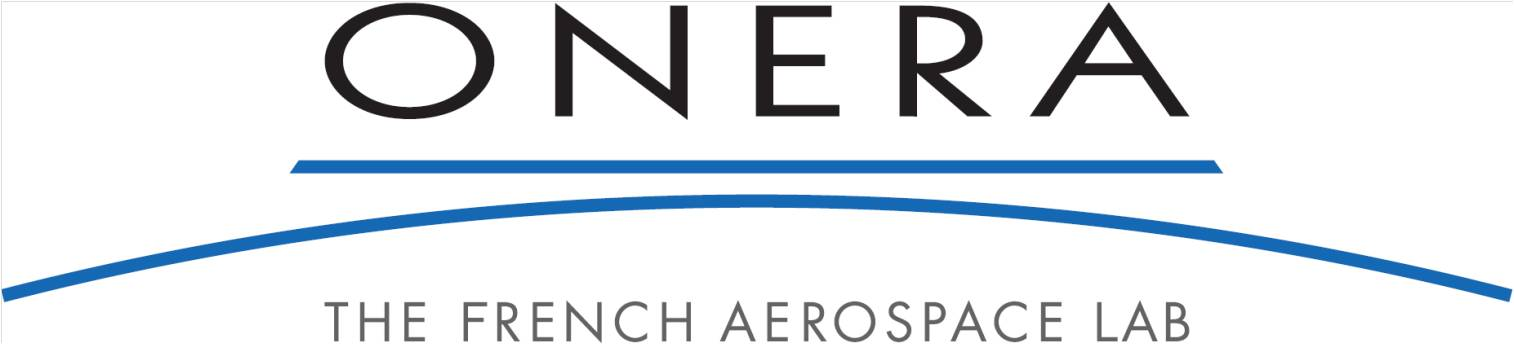
\includegraphics[scale=0.15]{ONERA_logo}\\

\includegraphics[scale=0.2]{logo_inria}
\end{tabular}

%\makebox[8em][r]{%
%\begin{minipage}{16em}
%\hfill
%\includegraphics[scale=0.1]{logo-lri}\\
%
\includegraphics[scale=0.1]{hd_logo_thales}\\
%\includegraphics[scale=0.05]{INRIA_CORPO_UK_CMJN}
%\end{minipage}
}


%%%%%%%%%%%%%%%%%%%%%%%%%%%%%%%%%%%%%%%%%%%%%%%%%%%%%%%%%%%%%%%%%%%%%%%%%%%%%%
%%% Now define the boxes that make up the poster
%%%---------------------------------------------------------------------------
%%% Each box has a name and can be placed absolutely or relatively.
%%% The only inconvenience is that you can only specify a relative position 
%%% towards an already declared box. So if you have a box attached to the 
%%% bottom, one to the top and a third one which should be in between, you 
%%% have to specify the top and bottom boxes before you specify the middle 
%%% box.
%%%%%%%%%%%%%%%%%%%%%%%%%%%%%%%%%%%%%%%%%%%%%%%%%%%%%%%%%%%%%%%%%%%%%%%%%%%%%%
    %
    % A coloured circle useful as a bullet with an adjustably strong filling
\newcommand{\colouredcircle}{%
\tikz{\useasboundingbox (-0.2em,-0.32em) rectangle(0.2em,0.32em); \draw[draw=black,fill=lightblue,line width=0.03em] (0,0) circle(0.18em);}}


%%%%%%%%%%%%%%%%%%%%%%%%%%%%%%%%%%%%%%%%%%%%%%%%%%%%%%%%%%%%%%%%%%%%%%%%
\headerbox{Motivation}{name=problem,column=0,row=0}{
%%%%%%%%%%%%%%%%%%%%%%%%%%%%%%%%%%%%%%%%%%%%%%%%%%%%%%%%%%%%%%%%%%%%%%%%

Real-world problems generally involve several \textcolor{purple}{\bf antagonistic objectives}, like makespan and cost for planning problems. The only approaches to multiobjective AI Planning rely on linear combinations of objectives, and metric sensitive planners, that are able to give different plans for different metrics, and hence to eventually approximate the \textcolor{purple}{\bf Pareto front} (i.e. the set of optimal trade-offs between the antagonistic objectives).

\vspace{0.3em}
}

%%%%%%%%%%%%%%%%%%%%%%%%%%%%%%%%%%%%%%%%%%%%%%%%%%%%%%%%%%%%%%%%%%%%%%%%
\headerbox{Multiobjective EA}{name=MOEA,column=0,below=problem}{
%%%%%%%%%%%%%%%%%%%%%%%%%%%%%%%%%%%%%%%%%%%%%%%%%%%%%%%%%%%%%%%%%%%%%%%%

Evolutionary Algorithms (EAs) are: metaheuristic \textcolor{purple}{\bf stochastic search}, using randomized mutations/crossovers to produce solutions and natural selection of the fittest.

The multiobjective method used here is an Indicator Based Evolutionary Algorithms, with the \textcolor{purple}{\bf hypervolume} indicator (\IBEAH).

\vspace{0.3em}
}

%%%%%%%%%%%%%%%%%%%%%%%%%%%%%%%%%%%%%%%%%%%%%%%%%%%%%%%%%%%%%%%%%%%%%%%%
\headerbox{Divide-and-Evolve}{name=DAE,column=0,below=MOEA}{
%%%%%%%%%%%%%%%%%%%%%%%%%%%%%%%%%%%%%%%%%%%%%%%%%%%%%%%%%%%%%%%%%%%%%%%%

Divide-and-Evolve (\DAE) is an evolutionary planner that embeds a classical planner and feeds it with a sequence of \textcolor{purple}{\bf subproblems}.

\begin{center}
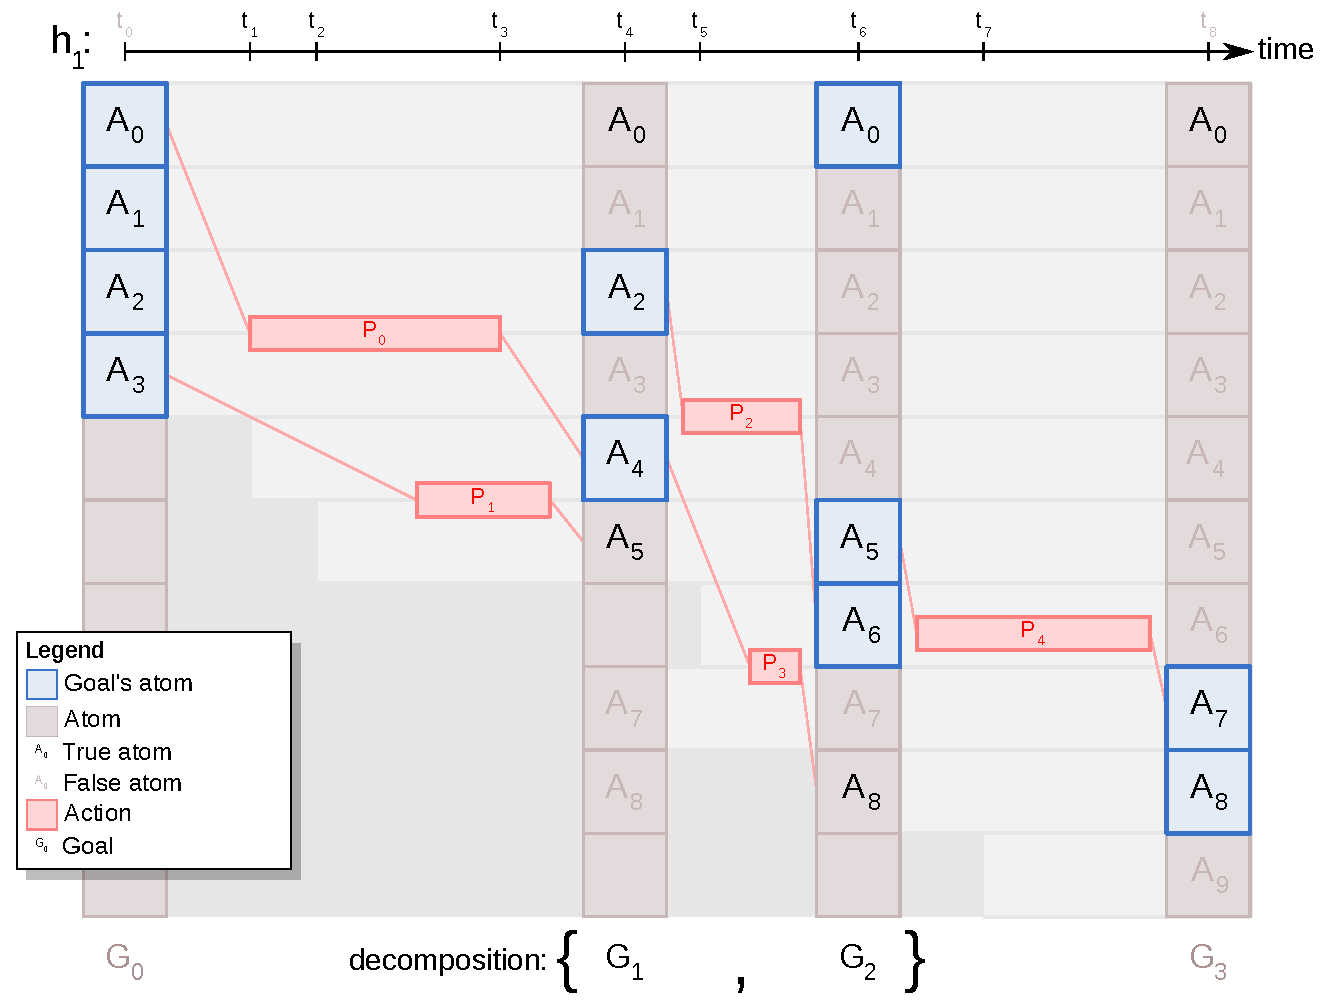
\includegraphics[width=1.0\textwidth]{DAEx}
% 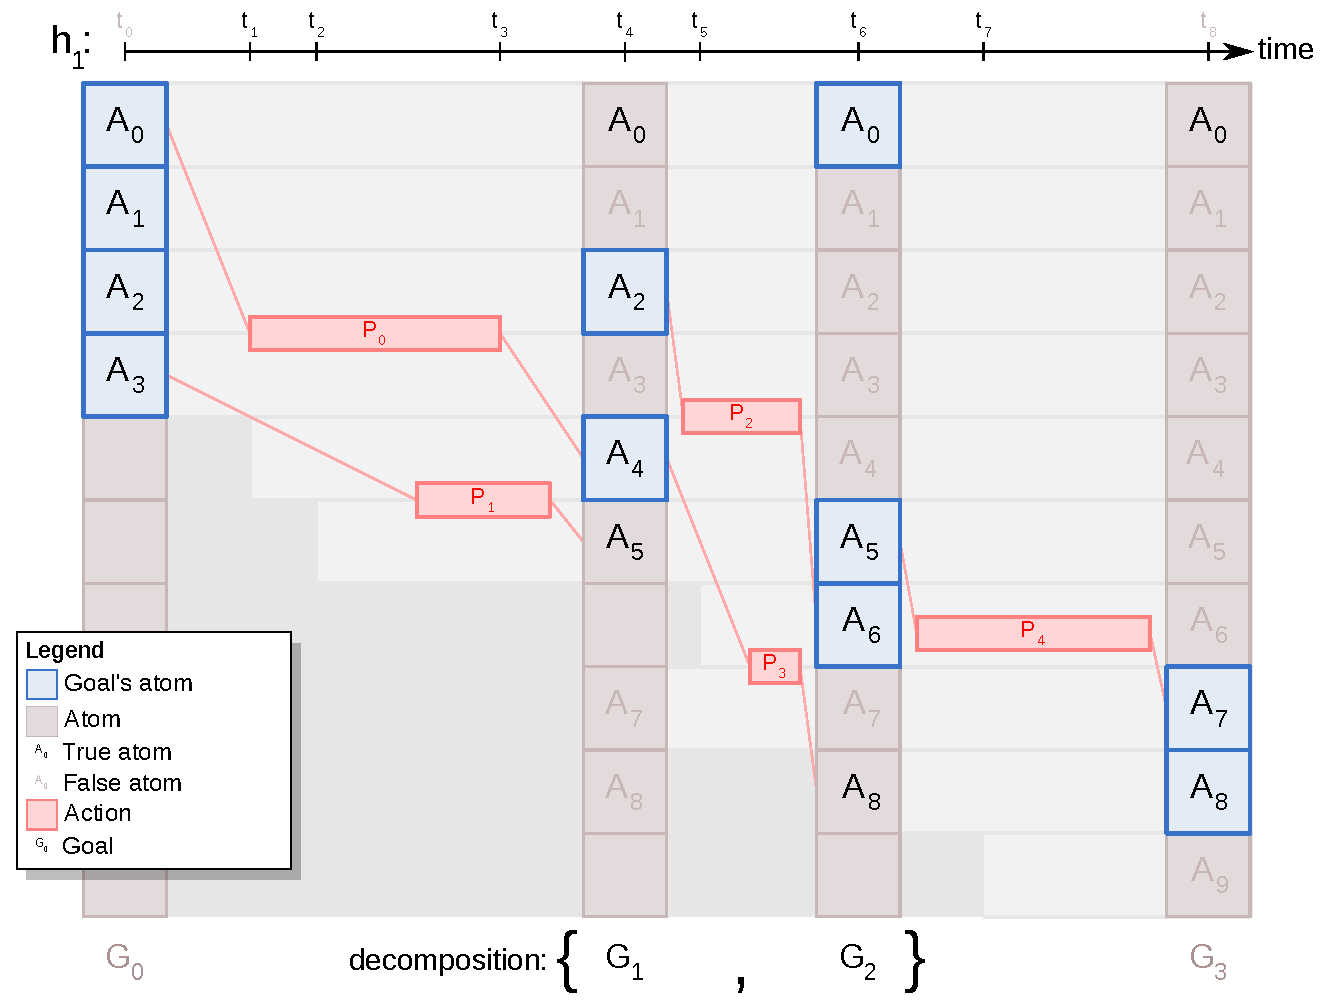
\includegraphics[scale=0.3]{DAEx}
\end{center}

\DAE\ can embed any existing planner. The lookahead heuristic-based satisficing planner \textcolor{purple}{\bf YAHSP}
%\cite{Vidal2004} 
has been demonstrated to be the best choice when used within \DAE.
%\cite{bibai-EvoCOP2010}

\vspace{0.3em}
}

%%%%%%%%%%%%%%%%%%%%%%%%%%%%%%%%%%%%%%%%%%%%%%%%%%%%%%%%%%%%%%%%%%%%%%%%
\headerbox{Benchmark Domains}{name=bench,column=0,below=DAE}{
%%%%%%%%%%%%%%%%%%%%%%%%%%%%%%%%%%%%%%%%%%%%%%%%%%%%%%%%%%%%%%%%%%%%%%%%

Highly simplified version of the well-known IPC domain \textcolor{purple}{\bf ZENOTRAVEL}, with the exact Pareto front:

\begin{center}
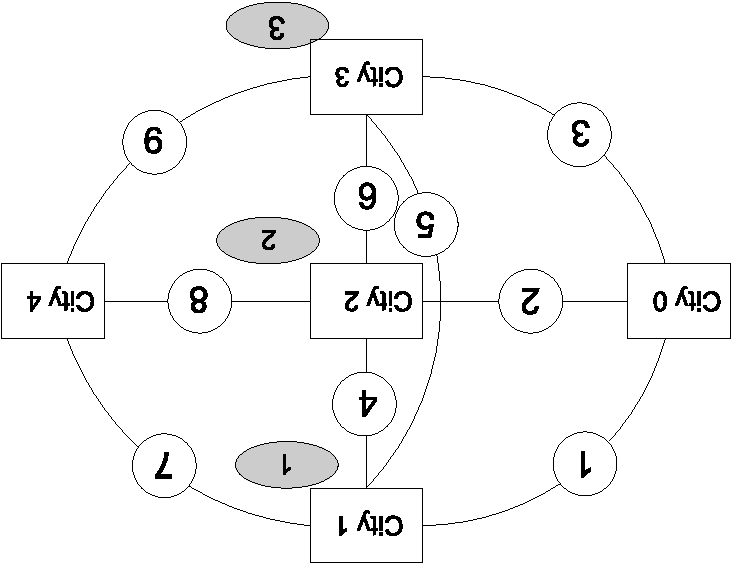
\includegraphics[width=0.75\textwidth,angle=180]{../figures/generiqueMiniMulti180}
\end{center}

Modifications of \textcolor{purple}{\bf IPC-2011 problems}:\\ \ELEVATORS, \FLOORTILE, \PARCPRINTER\ and \OPENSTACKS.

\vspace{0.3em}
}

%%%%%%%%%%%%%%%%%%%%%%%%%%%%%%%%%%%%%%%%%%%%%%%%%%%%%%%%%%%%%%%%%%%%%%%%
\headerbox{Multiobjective Divide-and-Evolve}{name=MODAE,column=1,span=2,row=0}{
%%%%%%%%%%%%%%%%%%%%%%%%%%%%%%%%%%%%%%%%%%%%%%%%%%%%%%%%%%%%%%%%%%%%%%%%

Two modifications of \DAEYAHSP\ are needed to turn it into a MOEA: \textcolor{purple}{\bf (i)} use a \textcolor{purple}{\bf multiobjective selection} (e.g. \IBEAH) in lieu of the tournament selection, \textcolor{purple}{\bf (ii)} use the embedded planner to compute both objectives (e.g., \textcolor{purple}{\bf makespan and cost}).

Because \YAHSP\ is both a temporal planner and a cost planner, two strategies are possible for \YAHSP\ within \MODAE: (i) it can be asked to optimize only the makespan (resp. the cost), (ii) to simply compute the cost (resp. the makespan) when executing the solution plan.

In \MODAEYAHSP, the choice between both strategies is governed by user-defined weights.
% , named respectively \WMAKESPAN\ and \WCOST. 
For each individual, the actual strategy is randomly chosen according to those weights, and applied to all subproblems of the individual.

\vspace{0.3em}
}


%%%%%%%%%%%%%%%%%%%%%%%%%%%%%%%%%%%%%%%%%%%%%%%%%%%%%%%%%%%%%%%%%%%%%%%%
\headerbox{Experiments}{name=experiments,column=1,span=2,below=MODAE}{
%%%%%%%%%%%%%%%%%%%%%%%%%%%%%%%%%%%%%%%%%%%%%%%%%%%%%%%%%%%%%%%%%%%%%%%%

\textcolor{purple}{\bf Parameter tuning} with \PARAMILS\ on one instance of moderate complexity in each domain. 11 independent runs of \textcolor{purple}{\bf 30  minutes} each. Implementation within the \textcolor{purple}{\bf ParadisEO-MOEO} framework, running on Xeon X5650@2.67GHz processors, on Ubuntu 10.04.

\vspace{0.3em}
}


%%%%%%%%%%%%%%%%%%%%%%%%%%%%%%%%%%%%%%%%%%%%%%%%%%%%%%%%%%%%%%%%%%%%%%%%
\headerbox{Results}{name=results,column=1,span=2,below=experiments}{
%%%%%%%%%%%%%%%%%%%%%%%%%%%%%%%%%%%%%%%%%%%%%%%%%%%%%%%%%%%%%%%%%%%%%%%%

% For \ZENOTRAVEL\ (simplified domains):
\begin{itemize}\compresslist
\item \MULTIZENO6\ instance: \MOLPG\ is only able to find a few points far away from the Pareto front. On the other hand, \MODAEYAHSP\ perfectly identifies the \textcolor{purple}{\bf complete Pareto front} in all runs for the ``Linear'' and ``Concave'' cases, while 2 runs out of 11 miss one point each in the ``Convex'' case.
\item \MULTIZENO9\ instance: while \MOLPG\ fails to find a single feasible plan, \MODAEYAHSP\ is able to approach the true Pareto front rather robustly.
\end{itemize}

\begin{center}
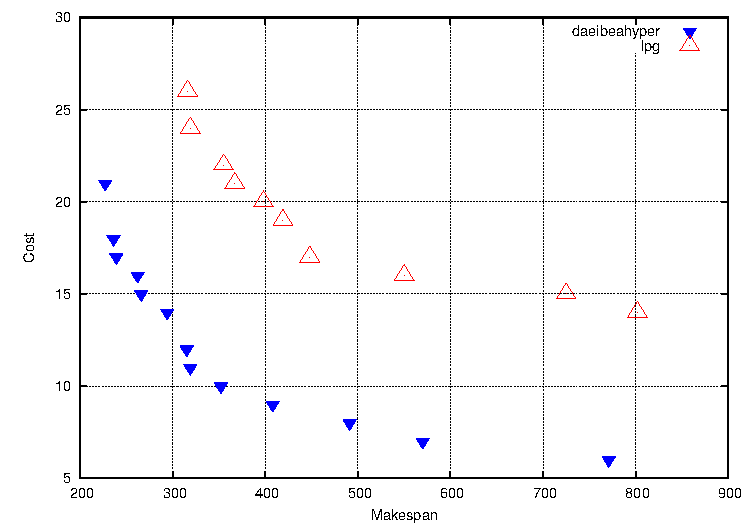
\includegraphics[scale=0.5]{p05_openstacks_Add_dae_pareto}  \hspace{1cm} 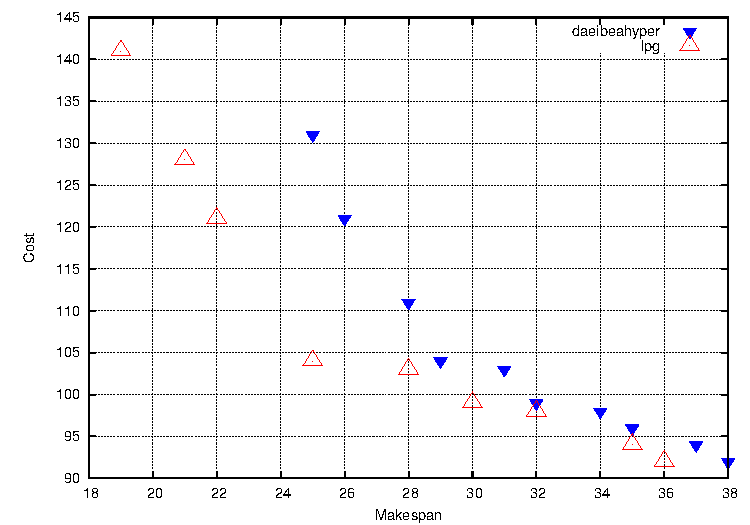
\includegraphics[scale=0.5]{pfile3_floortile_Add_dae_pareto}\\
\hspace{-3.cm} Openstacks5 \hspace{5.3cm} Floortile03 
\end{center}

% On multi-objectivized IPC-2011 instances:
\begin{itemize}\compresslist
\item \ELEVATORS\ 1, \MODAEYAHSP\ and \MOLPG\ find exactly the same Pareto front,
\item \ELEVATORS\ 5 and above, \MOLPG\ is unable to find any solution, \MODAEYAHSP\ identifies some Pareto front.
\item \OPENSTACKS\ 1, 5 and 10 (small instances) \MODAEYAHSP\ clearly finds a much better Pareto front than \MOLPG.
\item \OPENSTACKS\ 15 and 20, the situation is even worse for \MOLPG, that only finds very poor solutions (w.r.t. the ones found by \MODAEYAHSP).
\item \FLOORTILE\ 0, 3 and 4, \MOLPG\ outperforms \MODAEYAHSP. However, as the instance size increases (instance 4 and above), the gap between LPG and \DAE\ decreases.
\end{itemize}

\vspace{0.3em}
}



%%%%%%%%%%%%%%%%%%%%%%%%%%%%%%%%%%%%%%%%%%%%%%%%%%%%%%%%%%%%%%%%%%%%%%%%
\headerbox{Conclusion}{name=conclusion,column=1,span=2,below=results}{
%%%%%%%%%%%%%%%%%%%%%%%%%%%%%%%%%%%%%%%%%%%%%%%%%%%%%%%%%%%%%%%%%%%%%%%%

\MODAE\ approach can turn any planner into a multiobjective planner, provided it can reason on either objectives alone (e.g., the makespan and the cost), as has been done here with \YAHSP. The resulting algorithm is a truly Pareto-based multiobjective planner, that consistently outperforms the \MOLPG\ metric-based approach.

Meaningful multiobjective AI Planning benchmarks with gradual difficulties. The \MULTIZENO\ is a tunable artificial testbed, and was shown to be able to generate interesting Pareto fronts (e.g. convex with a knee as well as non-convex).

\vspace{0.3em}
}

%%%%%%%%%%%%%%%%%%%%%%%%%%%%%%%%%%%%%%%%%%%%%%%%%%%%%%%%%%%%%%%%%%%%%%%%
\headerbox{Acknowledgement}{name=acknowledgment,column=1,below=conclusion,span=1,above=bottom}{
%%%%%%%%%%%%%%%%%%%%%%%%%%%%%%%%%%%%%%%%%%%%%%%%%%%%%%%%%%%%%%%%%%%%%%%%
Work partially funded by the DESCARWIN ANR project (ANR-09-COSI-002).
}

%%%%%%%%%%%%%%%%%%%%%%%%%%%%%%%%%%%%%%%%%%%%%%%%%%%%%%%%%%%%%%%%%%%%%%%%
\headerbox{URL}{name=URL,column=2,below=conclusion,span=1,above=bottom}{
%%%%%%%%%%%%%%%%%%%%%%%%%%%%%%%%%%%%%%%%%%%%%%%%%%%%%%%%%%%%%%%%%%%%%%%%

\includegraphics[scale=0.1]{qr-code_url_johann_dreo_fr_png.pdf}
http://johann.dreo.fr/pro/
}



\end{poster}
\end{document}

